\subsection{Git Workflows}

In this section we detail the workflows available for the DHBB team to
adopt considering Git as a version control system for their files.

Git is a distributed version control system. It represents the current
official version of a project as a canonical repository of files. To
contribute to the project, one creates one's own public clone of the
project and push his changes to it. Then, one can send a request to
the project maintainer to pull in the changes implemented. One can add
the received repository as remote, test the changes locally, merge
them into their branch, and push back to their repository. The process
works as pictured in Figure~\ref{fig:git-model-1}.

\begin{figure}[thbp]
  \centering
  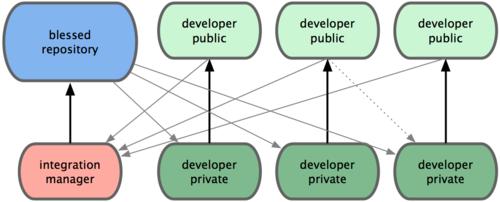
\includegraphics[width=.8\textwidth]{git-model-1.png}
  \caption{Integration-Manager Workflow}\label{fig:git-model-1}
\end{figure}

This is a very common workflow for developing projects in group, where
it is easy to fork a repository and push the changes into this fork
for everyone to see. One of the main advantages of this approach is
that one can continue to work, and the maintainer of the main
repository can pull in one's changes at any time. Contributors of the
DHBB for instance, would not have to wait for the DHBB coordinator to
incorporate their changes.

A variant of a multiple-repository workflow is shown in
Figure~\ref{fig:git-model-2}. It is generally used by huge projects
with hundreds of collaborators but can be adopted by DHBB. Various
integration managers are in charge of certain parts of the repository;
they are called lieutenants. All the lieutenants have one integration
manager known as the benevolent dictator. The benevolent dictator's
repository serves as the reference repository from which all the
collaborators need to pull.

\begin{figure}[thbp]
  \centering
  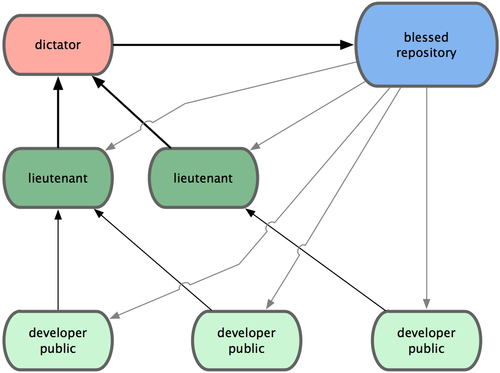
\includegraphics[width=.8\textwidth]{git-model-2.png}
  \caption{Dictator and Lieutenants Workflow}\label{fig:git-model-2}
\end{figure}

This kind of workflow is not common for git users but can be useful in
very big projects or in highly hierarchical environments, as it allows
the project leader (the dictator) to delegate much of the work and
collect large subsets of code at multiple points before integrating
them.

% These are some commonly used workflows that are possible with a
% distributed system like Git, but the reader can see that many
% variations are possible to suit your particular DHBB needs.

% Figure~\ref{fig:git} shows a possible git workflow. A more
% hierarchical workflow is also possible. The Git distributed version
% control system allows for handling this straightforwardly. The
% authors, responsible for creating the raw versions of historical
% data, would create markdown files. These files would then be revised
% by reviewers that submit their final versions to the coordinator or
% request authors revision. The coordinator is responsible for
% maintain the official DHBB git repository.


%%% Local Variables: 
%%% mode: latex
%%% TeX-master: "article_revA"
%%% End: 
